%%%%%%%%%%%%%%%%%%%%%%%%%%%%%%%%%%%%%%%%%
%
% CMPT 435
% Fall 2022
% Assignment 1
%
%%%%%%%%%%%%%%%%%%%%%%%%%%%%%%%%%%%%%%%%%

%%%%%%%%%%%%%%%%%%%%%%%%%%%%%%%%%%%%%%%%%
% Short Sectioned Assignment
% LaTeX Template
% Version 1.0 (5/5/12)
%
% This template has been downloaded from: http://www.LaTeXTemplates.com
% Original author: % Frits Wenneker (http://www.howtotex.com)
% License: CC BY-NC-SA 3.0 (http://creativecommons.org/licenses/by-nc-sa/3.0/)
% Modified by Alan G. Labouseur  - alan@labouseur.com
%
%%%%%%%%%%%%%%%%%%%%%%%%%%%%%%%%%%%%%%%%%

%----------------------------------------------------------------------------------------
%	PACKAGES AND OTHER DOCUMENT CONFIGURATIONS
%----------------------------------------------------------------------------------------

\documentclass[letterpaper, 10pt,DIV=13]{scrartcl} 

\usepackage[T1]{fontenc} % Use 8-bit encoding that has 256 glyphs
\usepackage[english]{babel} % English language/hyphenation
\usepackage{amsmath,amsfonts,amsthm,xfrac} % Math packages
\usepackage{sectsty} % Allows customizing section commands
\usepackage{graphicx}
\usepackage[lined,linesnumbered,commentsnumbered]{algorithm2e}
\usepackage{listings}
\usepackage{parskip}
\usepackage{lastpage}

\allsectionsfont{\normalfont\scshape} % Make all section titles in default font and small caps.

\usepackage{fancyhdr} % Custom headers and footers
\pagestyle{fancyplain} % Makes all pages in the document conform to the custom headers and footers

\fancyhead{} % No page header - if you want one, create it in the same way as the footers below
\fancyfoot[L]{} % Empty left footer
\fancyfoot[C]{} % Empty center footer
\fancyfoot[R]{page \thepage\ of \pageref{LastPage}} % Page numbering for right footer

\renewcommand{\headrulewidth}{0pt} % Remove header underlines
\renewcommand{\footrulewidth}{0pt} % Remove footer underlines
\setlength{\headheight}{13.6pt} % Customize the height of the header

\numberwithin{equation}{section} % Number equations within sections (i.e. 1.1, 1.2, 2.1, 2.2 instead of 1, 2, 3, 4)
\numberwithin{figure}{section} % Number figures within sections (i.e. 1.1, 1.2, 2.1, 2.2 instead of 1, 2, 3, 4)
\numberwithin{table}{section} % Number tables within sections (i.e. 1.1, 1.2, 2.1, 2.2 instead of 1, 2, 3, 4)

\setlength\parindent{0pt} % Removes all indentation from paragraphs.

\binoppenalty=3000
\relpenalty=3000

%----------------------------------------------------------------------------------------
%	TITLE SECTION
%----------------------------------------------------------------------------------------

\newcommand{\horrule}[1]{\rule{\linewidth}{#1}} % Create horizontal rule command with 1 argument of height

\title{	
   \normalfont \normalsize 
   \textsc{CMPT 435 - Fall 2022 - Dr. Labouseur} \\[10pt] % Header stuff.
   \horrule{0.5pt} \\[0.25cm] 	% Top horizontal rule
   \huge Assignment One  \\     	    % Assignment title
   \horrule{0.5pt} \\[0.25cm] 	% Bottom horizontal rule
}

\author{Josh Seligman \\ \normalsize joshua.seligman1@marist.edu}

\date{\normalsize\today} 	% Today's date.

\begin{document}
\maketitle % Print the title

\section{Singly Linked List}\label{linkedListSection}
\subsection{The Data Structure}\label{linkedListDataStructure}
A singly linked list is comprised of nodes which contain some form of data as well as a pointer to the next element within the list. As shown in 
Figure \ref{figure:linkedList}, the final node has a next of \textbf{null}, which marks the end of the list. In order to access a particular element,
one has to start at the beginning and traverse through the list until the desired node is found. This causes data access to be on the magnitude of $O(n)$ as the time required
to find an element has a linear relationship with the size of the list.

\begin{figure}[ht] 
    \centering 
    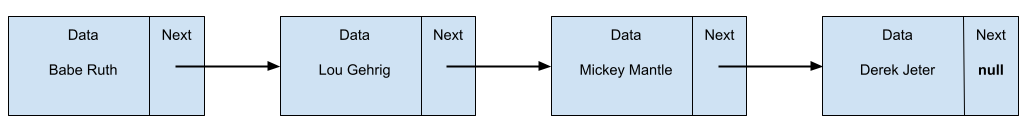
\includegraphics[width=15cm]{linkedList}
    \caption{Example singly linked list of 4 Yankees legends.}
    \label{figure:linkedList}
 \end{figure}

\subsection{Benefits of a Singly Linked List}
\subsubsection{Size}
As previously mentioned in Section \ref{linkedListDataStructure}, the last node within a linked list has a next of \textbf{null}. This characteristic enables linked lists to have no size restrictions barring memory capacity.
As a result, this feature makes linked lists preferred over arrays, which have a fixed length, when the size of the data is frequently changing and has an unkown maximum. For instance, as demonstrated in
Section \ref{mainProgramListing} starting on line 10 within \textit{main.cpp}, the size of the linked list is only limited by our needs and, if needed, more nodes are able
to easily be added to the list with their creation as done on lines 13-15 and linking as shown on lines 18 and 19. On the other hand, if the list was made with an array,
the size of the array would have to be provided at the time of the creation of the array, and it would not be easy to change the size if additional data have to be added
to the array.

\subsubsection{Data Type Flexibility}\label{linkedListDataType}
Linked lists do not have to be restricted to be able to store a specific data type. Instead, with the use of generics (C++ templates), the definition of a node is
independent of the data type that the user wants to store within the linked list. This provides flexibilty and reusability for many use cases. As demonstrated in
Section \ref{nodeListing} in \textit{node.h}, the definition of a node uses a generic T as the type of data being stored, which prevents any assumptions of the data
and ensures compatibility with all data types. However, due to how the C++ linker works and to prevent all the code from being written within a single header file,
the allowed types have to be stated on lines 13 and 14 of \textit{node.cpp}. This is a C++ specific issue and is not present in other languages such as Java.
Regardless, although they have to be specified for C++, any data type can still be stored within a node and a linked list. A demonstration of the user defining
which data type is stored in a node is in Section \ref{mainProgramListing} on lines 13-15 within \textit{main.cpp}. Instead of the Node class defining the data type,
the user is able to specify the type of data they want to store, which is a string in this situation but can be anything they want.

\section{Stack}
\subsection{The Data Structure}\label{stackDataStructure}
A stack uses a last in, first out (LIFO) approach to storing data. The most common analogy for stacks is a stack of plates. Each plate is
placed on top of each other to build the stack when being stored, but the plate on top is always the first to be used. In other words, the most recently plate
that was put away is also the first plate that is taken out. As displayed in Figure \ref{figure:stack}, the stack has a variable called top, which points to the first item in the stack.
Additionally, as shown by the arrows between each element, linked lists are used in the implementation of stacks. Stacks have 3 primary functions: push, pop, and isEmpty.
Push adds a new element to the top of the stack, pop removes the top item from the stack and returns the data, and isEmpty returns whether or not the stack is empty.

\begin{figure}[ht] 
    \centering 
    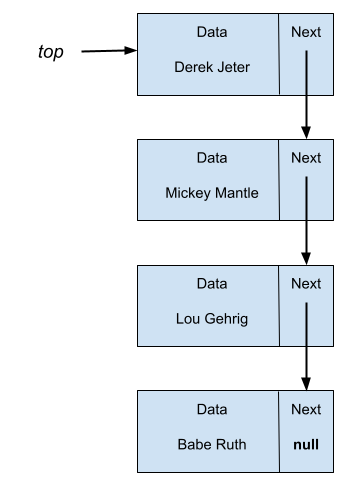
\includegraphics[height=8cm]{stack}
    \caption{Example stack of 4 Yankees legends.}
    \label{figure:stack}
 \end{figure}

\subsection{Benefits of a Stack}
\subsubsection{Time of Individual Data Access}
Stacks are incredibly fast when it comes to the implementation of the push and pop methods. As demonstrated in \textit{stack.cpp} in Section \ref{stackListing},
the push method on lines 21-28 creates the new node for the stack (line 24), points its next element to the current top of the stack (line 26), and then update the top of the stack to
point to the newly created node (line 28). These 3 steps will always run and do not depend on the current size of the stack, which means that the push method runs in $O(1)$ time.
The pop method on lines 30-46 is very similar in that it also executes the same few steps regardless of the current size of the stack. These steps are check if the stack is empty for safety (lines 33-36),
grab the data from the top of the stack (line 39), update the top pointer to point to the second item in the stack (line 40), and return the data (line 44). There is no need to traverse the list because the push
method made the new node the first element of the list, which is equivalent to the top of the stack. Therefore, just like the push method, the pop method also runs in $O(1)$ time.

\subsubsection{Compatibility with the Node Class}
As mentioned in Section \ref{stackDataStructure} and illustrated in Figure \ref{figure:stack}, the stack is implemented using a singly linked list. Therefore, the Stack
class in the code has to utilize the Node class written for singly linked lists, which can be found in Section \ref{nodeListing} and was analyzed in Section \ref{linkedListSection}.
In Section \ref{stackListing}, line 9 in \textit{stack.h} shows that the Stack class has an instance variable that points to the node on the top of the stack. Since the Node
class supports any data type (see Section \ref{linkedListDataType}), the Stack class has to be able to provide a data type for each node to store. For the same reasons as
described in Section \ref{linkedListDataType}, the Stack class also utilizes C++ templates to allow the user to decide which data type gets stored within the stack.
The Stack class is then able to take the data type that the user requests, such as \textbf{char} on line 32 of \textit{main.cpp} in Section \ref{mainProgramListing},
and pass it down to the data type that is stored within each node. This concept is demonstrated in Section \ref{stackListing} in \textit{stack.cpp} on 
line 24 when a new node is created and on line 9 of \textit{stack.h} when defining the top variable for the stack.

\section{Queue}
\subsection{The Data Structure}
A queue uses a first in, first out (FIFO) approach to handling data. One analogy to understand how a queue works is a line to buy movie tickets. The first person that
is in line for these tickets is the first to be assisted at the ticket counter. On the other hand, the last person to enter the line will also be the last one to
buy their ticket. Similar to stacks, queues are implemented using a singly linked list. As displayed in Figure \ref{figure:queue}, queues have a head variable 
that points to the first node within the linked list, which equates to the front of the line for the movie tickets. Queues have 3 primary functions: enqueue, dequeue,
and isEmpty. Enqueue adds a new element to the end of the queue, dequeue removes and returns the first element in the queue, and isEmpty checks to see if the queue is empty or not.

\begin{figure}[ht] 
    \centering 
    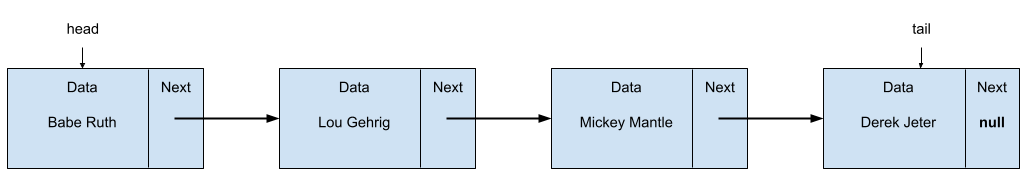
\includegraphics[width=15cm]{queue}
    \caption{Example queue of 4 Yankees legends.}
    \label{figure:queue}
 \end{figure}

\subsection{Benefits of a Queue}
\subsubsection{Compatibility with the Node Class}\label{queueNodes}
The Queue class, just like the Stack class, was implemented using templates to be able to support the use of the Node class, which requires an input of a data type upon
creation. As described in Section \ref{linkedListDataType}, C++ templates enable flexibilty and support for many different data types. Additionally, it is also very
safe to use because creating a Queue (or a Stack or Node) of a given type will result in a data structure that only accepts that type in the future. For instance, if a Queue is created
to support strings, one cannot attempt to enqueue an integer as there will be a type mismatch and the code will not compile. For instance, line 74 of \textit{main.cpp}
in Section \ref{mainProgramListing} is commented out because the compiler cannot convert a string to a single character, which causes a compilation error as the queue
cannot support the string.

\subsubsection{Error Safety}
In addition the the type safety of the templates as described in Section \ref{queueNodes}, the Queue class also has an error measure to prevent users from breaking
the program by doing something that is not allowed. In the case of the Queue class, the error safety occurs if the user tries to dequeue from an empty queue. As displayed on
lines 43-45 of \textit{queue.cpp} in Section \ref{queueListing}, the function checks if the queue is empty and throws an error if it is. This is really important
as, without the check, there would be a runtime error that crashes the program from attempting to work with a null pointer. In the test program for the queue in \textit{main.cpp} of
Section \ref{mainProgramListing}, lines 67-72 use a try-catch block to make sure the programmed error is thrown when attempting to dequeue from an
empty queue. It is of importance to note that this feature is also implemented in the Stack class when attempting to pop from an empty stack (see lines 
33-35 of \textit{stack.cpp} in Section \ref{stackListing}).

\section{Main Program}
\subsection{Program Overview}

\subsection{Good Parts of the Program}

%----------------------------------------------------------------------------------------
%   start PROBLEM ONE
%----------------------------------------------------------------------------------------
% \section{Problem One}

% \subsection{The Data Structure}
% An $n$-element array of integer pairs: ($currentCount$, $predecessorSum$) will, once initialized in the preprocessing step,  support \textsc{Member}, \textsc{Less}, and \textsc{Range} operations as described in Section \ref{operations} in $O(1)$ (constant) time.

% For illustration, consider the case where $S = (1, 2, 3, 4, 7, 7, 7, 7, 7, 8, 9, 10, 10,10,10,10,10, 14, 16)$. \\
% Here we have $m = 19$ elements in $S$ ranging in value from 1 through $n = 16$.
% The array for $S$ after preprocessing is given in Figure~\ref{figure:array}.

% % This is how we include a figure when 
% % the file is in the same directory as this document.
% \begin{figure}[ht] 
%    \centering 
% %    \includegraphics[width=11cm]{array}
%    \caption{Example array built from 19 values, 10 of them unique.}
%    \label{figure:array}
% \end{figure}

% \subsection{Preprocessing}
% There are two preprocessing steps, \textsc{Tally} and \textsc{Predecessor Sum}, each of which is $O(m+n)$ as we will see in Equations \ref{equation:pass1} and \ref{equation:pass2} below.
% This makes the overall performance $O(m+n)$ because 
% $2 \cdot O(m+n) =\footnote{This is an abuse of the notation, but if it's okay in the CLRS~\cite{clrs} book I hope it's okay here.} O(m+n)$.

% % Note bot the footnote and the citation in the above two lines.

% \subsubsection{Pass one: Tally}
% For each element $i$ in $S$ we'll store its number of occurrences at $A[i].currentCount$.

% % This is an example of including an algorithm in your document.
% \begin{algorithm}[H]
%     \SetAlgoLined
%     \caption{Tally}
%     \label{algorithm:tally}
%     \KwData{collection $S$}
%     \KwResult{array $A$ containing tallys for each element $i$ in $S$ }
   
%     allocate $A[n]$\;
%     \For{$j \leftarrow 1$ \KwTo $n$}{
%          $A[j].currentCount \leftarrow 0$\;
%     }   
%     \ForEach(// There are $m$ elements in $s$.){element i in S}{
%          $A[i].currentCount \leftarrow A[i].currentCount + 1$\;
%     }
% \end{algorithm}

% \textbf{Asymptotic Analysis} \\
% We are given $m$ integer values (the size of the collection), each in the range $[1..n]$ (the size of the domain) and want to iterate over them, computing the tally for each.
% Consider Algorithm~\ref{algorithm:tally}.
% Line 1 executes in constant time.
% Lines 2 through 4 execute in $O(n)$ time because we are iterating from 1 to $n$.  
% Lines 5 through 7 execute in $O(m)$ time because we are iterating over all the elements of $S$, of which there are $m$.  

% % This is how you include an equation:

% So, for pass one, we have :
% \begin{equation}   
%    \label{equation:pass1}   
%    \begin{split}
%    O(pass1) & = constant + O(n) + O(m)\\
%             & = O(n) + O(m)\\
%             & = O(m+n)   
%    \end{split}
% \end{equation}

% \subsubsection{Pass two: Predecessor Sum}
% Once the tally is done we need to make another pass over $A$ to compute, for each $A[i] : i>1$, 
% the sum of all of its predecessors ($A[1] .. A[i-1]$) and store that in $A[i].predecessorSum$.

% \begin{algorithm}[H]
%     \SetAlgoLined
%     \caption{Predecessor Sum}
%     \label{algorithm:predecessorSum}
%     \KwData{array $A$ containing tallys for each element $i$ in $S$}
%     \KwResult{a new and improved array $A$, now with the predecessor sums}
   
%     $A[1].predecessorSum \leftarrow 0$\;
%    \If {n > 1} {
%        \For{$k\leftarrow 2$ \KwTo $n$}{
%             $A[k].predecessorSum \leftarrow A[k-1].predecessorSum + A[k-1].currentCount$\;
%         }   
%    }
% \end{algorithm}

% \textbf{Asymptotic Analysis}\\
% Looking at Algorithm~\ref{algorithm:predecessorSum}, line 1 is assignment, a constant time operation.
% If lines 3 through 5 execute at all, they do so in $O(n)$ time because we make $n - 1$ iterations over line 4, which is assignment and array lookups, both constant time operations.
% For pass two, we have :
% \begin{equation}
%    \label{equation:pass2}   
%    \begin{split}       
%        O(pass2) & = constant + O(n) \\
%                 & = O(n) \\
%                 & = O(m+n) \, \text{which is ok so long as $m > 0$}   
%     \end{split}
% \end{equation}


% \subsection{Operations}\label{operations}

% \subsubsection{Member}

% \begin{algorithm}[H]
%     \SetAlgoLined
%     \caption{Member}
%     \label{algorithm:member}
%     \KwIn{parameter $i$}
%     \KwData{a new and improved array $A$, replete with tallys and predecessor sums}
%     \KwOut{$True$ if $i$ exists in $S$, $False$ otherwise}
     
%     \eIf {$(i \ge 1) \land (i \le n)$} {
%         return $(A[i].currentCount > 0)$\;
%     } {
%         return $False$\;
%    }
% \end{algorithm}

% \textbf{Asymptotic Analysis}\\
% Looking at Algorithm~\ref{algorithm:member}, line 1 consists of comparisons, which are constant time operations.
% Line 2 is an array lookup and a comparison, both constant time operations.
% The remaining parts of the algorithm (including the rest of line 2) are for program control, and not considered in this analysis. Since all parts of the algorithm execute in constant time, the whole thing executes in constant time and is therefore $O(1)$.

% \subsubsection{Less}

% \begin{algorithm}[H]
%     \SetAlgoLined
%     \caption{Less}
%     \label{algorithm:less}
%     \KwIn{parameter $i$}
%     \KwData{a new and improved array $A$, replete with tallys and predecessor sums}
%     \KwOut{The number of elements in $S$ that are strictly less than $i$.}
     
%     \eIf {$(i \ge 1) \land (i \le n)$} {
%         return $A[i].predecessorSum$\;
%     } {
%         return 0\;
%    }
% \end{algorithm}

% \textbf{Asymptotic Analysis}\\
% Looking at Algorithm~\ref{algorithm:less}, line 1 consists of comparisons, which are constant time operations.
% Line 2 is an array lookup, a constant time operation.
% The remaining parts of the algorithm (including the rest of line 2) are for program control, and not considered in this analysis. Since all parts of the algorithm execute in constant time, the whole thing executes in constant time, and is therefore $O(1)$.

% \subsubsection{Range}

% \begin{algorithm}[H]
%     \SetAlgoLined
%     \caption{Range}
%     \label{algorithm:range}
%     \KwIn{parameters $i$ and $j$ : $i \le j$}
%     \KwData{a new and improved array $A$, replete with tallys and predecessor sums}
%     \KwOut{The number of elements in $S$ that are in the range $[i .. j]$.}
     
%     \eIf {$(i \ge 1) \land (i \le n) \land (j \ge 1) \land (j \le n) \land (i \le j)$} {
%         return $(A[j].currentCount + A[j].predecessorSum - A[i].predecessorSum)$\;
%     } {
%         return 0\;
%    }
% \end{algorithm}

% \textbf{Asymptotic Analysis}\\
% Looking at Algorithm~\ref{algorithm:range}, line 1 consists of comparisons, which are constant time operations.
% Line 2 consists of array lookups, addition, and subtraction, all constant time operations.
% The remaining parts of the algorithm (including the rest of line 2) are for program control, and not considered in this analysis. Since all parts of the algorithm execute in constant time, the whole thing executes in constant time, and is therefore $O(1)$.

% %----------------------------------------------------------------------------------------
% %   end PROBLEM ONE
% %----------------------------------------------------------------------------------------

% \pagebreak

% %----------------------------------------------------------------------------------------
% %   start PROBLEM TWO
% %----------------------------------------------------------------------------------------
% \section{Problem Two}

% %----------------------------------------------------------------------------------------
% %   end PROBLEM Two
% %----------------------------------------------------------------------------------------

% \pagebreak

% %----------------------------------------------------------------------------------------
% %   start PROBLEM Three
% %----------------------------------------------------------------------------------------
% \section{Problem Three}

% %----------------------------------------------------------------------------------------
% %   end PROBLEM THREE
% %----------------------------------------------------------------------------------------

% \pagebreak

% %----------------------------------------------------------------------------------------
% %   REFERENCES
% %----------------------------------------------------------------------------------------
% % The following two commands are all you need in the initial runs of your .tex file to
% % produce the bibliography for the citations in your paper.
% \bibliographystyle{abbrv}
% \bibliography{lab01} 
% % You must have a proper ".bib" file and remember to run:
% % latex bibtex latex latex
% % to resolve all references.

% \pagebreak

%----------------------------------------------------------------------------------------
%   Appendix
%----------------------------------------------------------------------------------------

\section{Appendix}
\lstset{numbers=left, numberstyle=\tiny, stepnumber=1, numbersep=5pt, basicstyle=\footnotesize\ttfamily}

\subsection{Singly Linked List}\label{nodeListing}
\subitem{node.cpp}
\begin{lstlisting}[frame=single, ]  
#include <string>

#include "node.h"

template <typename T>
Node<T>::Node(T initialData) {
    // Initialize the node with the data and without a next node in the linked list
    Node::data = initialData;
    Node::next = nullptr;
}

// Define acceptable data types that the Node can accept for the template
template class Node<std::string>;
template class Node<char>;
\end{lstlisting}

\subitem{node.h}
\begin{lstlisting}[frame=single, ]  
#pragma once

// Node represents an item within a singly linked list and can store data of a given type
template <typename T>
class Node {
    public:
        // A node has the data it is storing (of a type defined by the user)
        // and a pointer to the next node
        T data;

        // The pointer uses the template to make sure all elements of the linked list
        // store the same data type
        Node<T>* next;

        // Nodes will be instantiated with some data and not have a next node
        Node(T initialData);
};

// Super helpful resource on templates for c++
// https://isocpp.org/wiki/faq/templates#separate-template-fn-defn-from-decl
\end{lstlisting}

\subsection{Stack}\label{stackListing}
\subitem{stack.cpp}
\begin{lstlisting}[frame=single, ]  
#include <string>

#include "stack.h"
#include "node.h"

// Instantiate the stack with the top pointing to nothing
template <typename T>
Stack<T>::Stack() {
    top = nullptr;
}

template <typename T>
Stack<T>::~Stack() {
    // Since the nodes were created on the heap, we have to
    // make sure everything is cleared from memory
    while (!isEmpty()) {
        pop();
    }
}

// Creates a new node and adds it to the stack
template <typename T>
void Stack<T>::push(T newData) {
    Node<T>* newNode = new Node(newData);
    // Set the next first so we do not lose the rest of the stack
    newNode->next = top;
    top = newNode;
}

// Removes the top node from the stack
template <typename T>
T Stack<T>::pop() {
    if (isEmpty()) {
        // Throw an exception if the stack is already empty
        throw std::invalid_argument("Tried to pop from an empty stack.");
    } else {
        // We need to collect the data in the node before removing it from the stack
        Node<T>* topNode = top;
        T topData = topNode->data;
        top = top->next;

        // Since the node was created on the heap, we have to free it from memory
        delete topNode;
        return topData;
    }
}

// Checks to see if the stack is empty or not
template <typename T>
bool Stack<T>::isEmpty() {
    return top == nullptr;
}

// Define acceptable data types that the Stack can accept for the template
template class Stack<std::string>;
template class Stack<char>;
\end{lstlisting}

\subitem{stack.h}
\begin{lstlisting}[frame=single, ]  
#pragma once

#include "node.h"

template <typename T>
class Stack {
private:
    // Top points to the top of the stack
    Node<T>* top;
public:
    // We need a constructor and destructor
    Stack();
    ~Stack();

    // Push adds a new element to the stack
    void push(T newData);

    // Pop removes the top element from the stack
    T pop();

    // isEmpty checks to see if the stack is empty
    bool isEmpty();
};
\end{lstlisting}

\subsection{Queue}\label{queueListing}
\subitem{queue.cpp}
\begin{lstlisting}[frame=single, ]  
#include <string>

#include "queue.h"
#include "node.h"

// Instantiate the queue with the head pointing to nothing
template <typename T>
Queue<T>::Queue() {
    head = nullptr;
}

template <typename T>
Queue<T>::~Queue() {
    // Since the nodes were created on the heap, we have to
    // make sure everything is cleared from memory
    while (!isEmpty()) {
        dequeue();
    }
}

// Creates a new node and adds it to the queue
template <typename T>
void Queue<T>::enqueue(T newData) {
    Node<T>* newNode = new Node(newData);
    
    if (isEmpty()) {
        // Immediately set the head to be the new node if we are empty
        head = newNode;
    } else {
        // Traverse to the back of the queue
        Node<T>* cur = head;
        while (cur->next != nullptr) {
            cur = cur->next;
        }
        // Insert the new node in the back of the queue
        cur->next = newNode;
    }
}

// Removes the front node from the queue
template <typename T>
T Queue<T>::dequeue() {
    if (isEmpty()) {
        // Throw an exception if the queue is already empty
        throw std::invalid_argument("Tried to dequeue from an empty queue.");
    } else {
        // We need to collect the data in the node before removing it from the queue
        Node<T>* frontNode = head;
        T frontData = frontNode->data;
        head = head->next;

        // Since the node was created on the heap, we have to free it from memory
        delete frontNode;
        return frontData;
    }
}

// Checks to see if the queue is empty or not
template <typename T>
bool Queue<T>::isEmpty() {
    return head == nullptr;
}

// Define acceptable data types that the Queue can accept for the template
template class Queue<std::string>;
template class Queue<char>;
\end{lstlisting}

\subitem{queue.h}
\begin{lstlisting}[frame=single, ]  
#pragma once

#include "node.h"

template <typename T>
class Queue {
private:
    // Head points to the front of the queue
    Node<T>* head;
public:
    // We need a constructor and destructor
    Queue();
    ~Queue();

    // Enqueue adds a new element to the queue
    void enqueue(T newData);

    // Dequeue removes the front element from the queue
    T dequeue();

    // isEmpty checks to see if the queue is empty
    bool isEmpty();
};
\end{lstlisting}

\subsection{Main Program}\label{mainProgramListing}
\subitem{main.cpp}
\begin{lstlisting}[frame=single, ]  
#include <iostream>
#include <string>

#include "node.h"
#include "stack.h"
#include "queue.h"
#include "fileUtil.h"
#include "util.h"

// Function to test the Node class
void testNode() {
    // Create the nodes on the stack, so we do not have to delete later
    Node<std::string> n1("node 1");
    Node<std::string> n2("node 2");
    Node<std::string> n3("node 3");

    // Set up the links
    n1.next = &n2;
    n2.next = &n3;

    // Print out the data of each node in the linked list
    Node<std::string>* cur = &n1;
    while (cur != nullptr) {
        std::cout << cur->data << std::endl;
        cur = cur->next;
    }
}

// Function to test the Stack class
void testStack() {
    // Create a stack and add some data to it
    Stack<char> stack;
    stack.push('h');
    stack.push('s');
    stack.push('o');
    stack.push('J');

    // Print out the letters as we remove them from the stack
    while (!stack.isEmpty()) {
        std::cout << stack.pop();
    }
    std::cout << std::endl;

    try {
        // This should throw an error
        stack.pop();
    } catch (const std::invalid_argument& e) {
        std::cerr << e.what() << std::endl;
    }
}

// Function to test the Queue class
void testQueue() {
    // Create a queue and add some data to it
    Queue<char> queue;
    queue.enqueue('J');
    queue.enqueue('o');
    queue.enqueue('s');
    queue.enqueue('h');

    // Print out the letters as we remove them from the queue
    while (!queue.isEmpty()) {
        std::cout << queue.dequeue();
    }
    std::cout << std::endl;

    try {
        // This should throw an error
        queue.dequeue();
    } catch (const std::invalid_argument& e) {
        std::cerr << e.what() << std::endl;
    }

    // queue.enqueue("Hello");
}

// Function to check if a string is a palindrome, minus whitespace and capitalization
bool isPalindrome(std::string word) {
    // Initialize an empty stack and queue for the checks
    Stack<char> wordStack;
    Queue<char> wordQueue;

    // Iterate through each character in the word to populate the stack and queue
    for (int i = 0; i < word.length(); i++) {
        char character = word[i];
        if (character == ' ') {
            // Go to next character because we are ignoring whitespace
            continue;
        } else if (character >= 'a' && character <= 'z') {
            // Adjust the character to make it uppercase by taking the difference between
            // the start of the lowercase letters and the start of the uppercase letters
            character -= 'a' - 'A';
        }
        // Add the character to both the stack and the queue
        wordStack.push(character);
        wordQueue.enqueue(character);
    }

    while (!wordStack.isEmpty() && !wordQueue.isEmpty()) {
        // Get the character from the top of the stack and queue
        char charFromStack = wordStack.pop();
        char charFromQueue = wordQueue.dequeue();

        if (charFromStack != charFromQueue) {
            // We can return false because we already know that
            // the string is not a palindrome
            return false;
        }
    }

    // The string is a palindrome
    return true;
}

int main() {
    std::cout << "----- Testing Node class -----" << std::endl;
    testNode();
    std::cout << std::endl;

    std::cout << "----- Testing Stack class -----" << std::endl;
    testStack();
    std::cout << std::endl;

    std::cout << "----- Testing Queue class -----" << std::endl;
    testQueue();
    std::cout << std::endl;

    std::cout << "----- Testing isPalindrome -----" << std::endl;
    std::cout << isPalindrome("racecar") << std::endl; // 1
    std::cout << isPalindrome("RaCecAr") << std::endl; // 1
    std::cout << isPalindrome("ra   c e   car") << std::endl; // 1
    std::cout << isPalindrome("4") << std::endl; // 1
    std::cout << isPalindrome("") << std::endl; // 1
    std::cout << isPalindrome("ABC") << std::endl; // 0
    std::cout << std::endl;

    std::cout << "----- Magic Items -----" << std::endl;
    try {
        // Read the file and store it in an array
        StringArr* data = readFile("magicitems.txt");

        // Only print out the palindromes
        for (int i = 0; i < data->length; i++) {
            if (isPalindrome(data->arr[i])) {
                std::cout << data->arr[i] << std::endl;
            }
        }

        // Clean up memory
        delete data;
    } catch (const std::invalid_argument& e) {
        std::cerr << e.what() << std::endl;
    }

    return 0;
}
\end{lstlisting}

\end{document}